% ============================================================
%  第3章：模型设计与实现
% ============================================================
\chapter{模型设计与实现}

\section{整体架构设计}

本文模型整体沿用了 Transformer 的编码器-解码器结构\cite{vaswani2017attention}，但在注意力计算与位置编码两方面进行了针对性改进。

\zhlipsum[1]

\begin{figure}[ht]
\centering
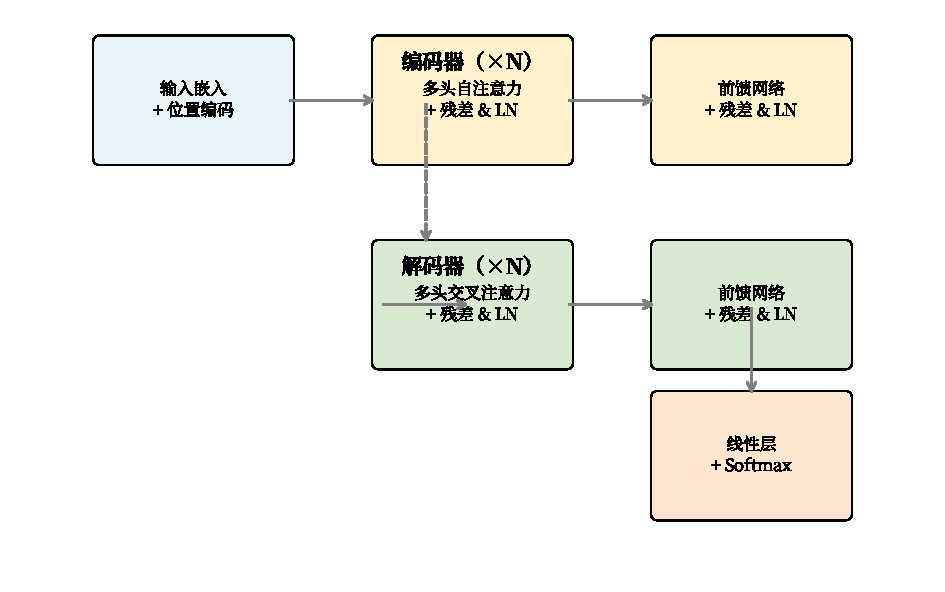
\includegraphics[width=0.85\textwidth]{figures/example_architecture.pdf}
\caption{模型整体架构}
\label{fig:architecture}
\end{figure}

\safeSectionBreak

\section{稀疏注意力模块}

\zhlipsum[3]

设输入序列长度为$n$，标准自注意力的计算复杂度为$O(n^2 \cdot d)$。通过引入稀疏掩码矩阵$M \in \{0, 1\}^{n \times n}$，可以将注意力限制在局部窗口内：
\begin{equation}
  \text{SparseAttn}(Q, K, V) = \text{softmax}\!\left(\frac{QK^{T}}{\sqrt{d_k}} \odot M\right) V
  \label{eq:sparse_attn}
\end{equation}
其中$M_{ij} = 1$当且仅当$|i - j| \leq w$，复杂度降为$O(n \cdot w \cdot d)$。该思路与原始 Transformer\cite{vaswani2017attention} 中提出的注意力模式一脉相承，但通过引入结构化稀疏显著提升了长序列处理效率。

\section{混合编码策略}

\zhlipsum[5]

位置编码采用可学习嵌入与正弦编码的混合方案：
\begin{align}
  \text{PE}(pos, 2i) &= \sin\left(\frac{pos}{10000^{2i/d_{\text{model}}}}\right) \\
  \text{PE}(pos, 2i+1) &= \cos\left(\frac{pos}{10000^{2i/d_{\text{model}}}}\right)
\end{align}

与 BERT\cite{devlin2019bert} 仅使用单一位置编码不同，本文的输入嵌入为词嵌入、位置编码与段嵌入三者之和：
\begin{equation}
  E_{\text{input}} = E_{\text{token}} + \text{PE}(pos) + E_{\text{segment}}
  \label{eq:input_emb}
\end{equation}

\safeSectionBreak

\section{训练策略}

\zhlipsum[8]

训练目标为最小化交叉熵损失：
\begin{equation}
  \mathcal{L} = -\frac{1}{N} \sum_{i=1}^{N} \sum_{t=1}^{T} \log P(y_t^{(i)} \mid y_{<t}^{(i)}, x^{(i)})
  \label{eq:loss}
\end{equation}

\safeFloatGap

\begin{figure}[h]
\centering
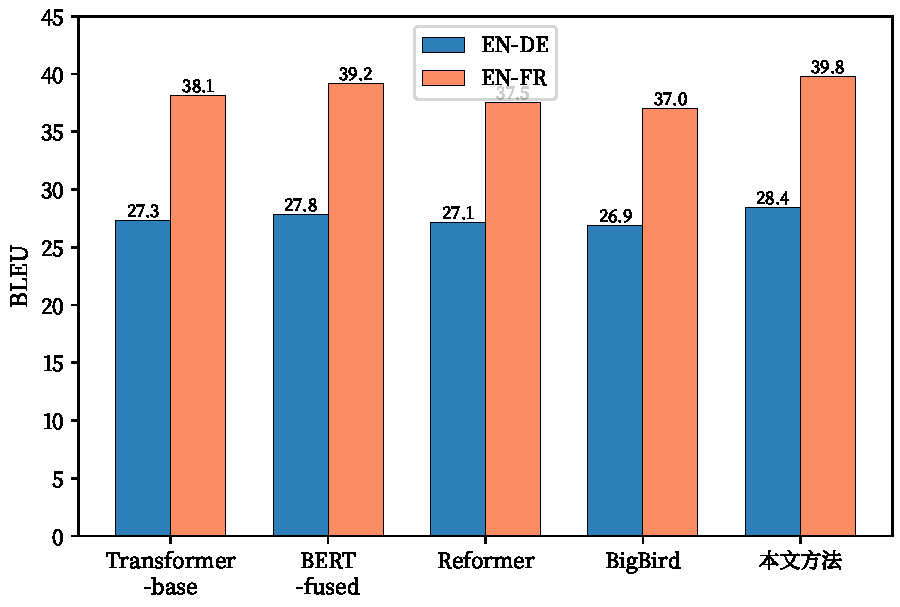
\includegraphics[width=0.75\textwidth]{figures/example_bar.pdf}
\caption{不同配置下的模型性能对比}
\label{fig:config_comparison}
\end{figure}
